\documentclass{article}

\usepackage{amsmath,geometry,amsfonts,array,makecell,enumitem,bm,esint,booktabs,multirow,mathtools,upgreek,amssymb,pgfplots,mathrsfs}
\usepackage[amsmath]{ntheorem}
\usepackage[hidelinks,naturalnames]{hyperref}
\usepackage[nameinlink,noabbrev]{cleveref}
\usepackage{fancyhdr}
\pagestyle{fancy}
\fancyhead[L]{\itshape\nouppercase{\leftmark}}
\fancyhead[R]{Ring Polymer Molecular Dynamics}

\title{Ring_Polymer}
\author{Yue Wu}

\geometry{a4paper,hmargin=1.1in,vmargin=1.2in}

\setlength{\parskip}{1em}
\tolerance=1000
\emergencystretch=1em
\hyphenpenalty=1000
\exhyphenpenalty=100
\righthyphenmin=3

\pgfplotsset{compat=1.18}

\theoremstyle{plain}\theoremheaderfont{\normalfont\itshape}\theorembodyfont{\rmfamily}\theoremseparator{.}\newtheorem*{rem}{Remark}\newtheorem*{ex}{Example}\newtheorem*{proof}{Proof}\newtheorem*{altp}{Alternative proof}

\theoremstyle{plain}\theoremheaderfont{\normalfont\bfseries}\theorembodyfont{\rmfamily}\theoremseparator{.}\newtheorem{thm}{Theorem}[section]\newtheorem{lem}[thm]{Lemma}\newtheorem{prop}[thm]{Proposition}\newtheorem*{cor}{Corollary}\newtheorem{defn}[thm]{Definition}\newtheorem{clm}[thm]{Claim}\newtheorem{clminproof}{Claim}

\theoremstyle{break}\theoremheaderfont{\normalfont\itshape}\theorembodyfont{\rmfamily}\theoremseparator{.\medskip}\newtheorem*{proofskip}{Proof}\newtheorem*{exs}{Examples}\newtheorem*{rems}{Remarks}

\theoremstyle{break}\theoremheaderfont{\normalfont\bfseries}\theorembodyfont{\rmfamily}\theoremseparator{.\medskip}\newtheorem{lemskip}[thm]{Lemma}\newtheorem{defnskip}[thm]{Definition}\newtheorem{propskip}[thm]{Proposition}\newtheorem{thmskip}[thm]{Theorem}

\crefname{thm}{Theorem}{Theorems}\crefname{defn}{Definition}{Definitions}\crefname{lem}{Lemma}{Lemmas}\crefname{lemskip}{Lemma}{Lemmas}\crefname{cor}{Corollary}{Corollaries} \crefname{prop}{Proposition}{Propositions}\crefname{clm}{Claim}{Claims}

\setcounter{tocdepth}{2}
\setcounter{section}{0}
\numberwithin{equation}{section}

\newcommand{\qed}{\hfill\ensuremath{\Box}}
\newcommand{\unit}[1]{\ \mathrm{#1}}
\newcommand{\ii}{\mathrm{i}}
\newcommand{\ee}{\mathrm{e}}
\newcommand{\tp}{^\mathrm{T}}
\newcommand{\dd}[2][]{\mathrm{d}^{#1} #2\,}
\newcommand{\DD}[1]{D #1\,}
\renewcommand{\d}[2][]{\mathrm{d}^{#1} #2}
\newcommand{\dv}[3][]{\frac{\mathrm{d}^{#1} #2}{{\mathrm{d} #3}^{#1}}}
\newcommand{\pdv}[3][]{\frac{\partial^{#1} #2}{{\partial #3}^{#1}}}
\newcommand{\bra}[1]{\left\langle #1 \right|}
\newcommand{\ket}[1]{\left| #1 \right\rangle}
\newcommand{\braket}[2]{\left\langle #1 \middle| #2 \right\rangle}
\newcommand{\mel}[3]{\left\langle #1 \middle| #2 \middle| #3 \right\rangle}
\newcommand{\redmel}[3]{\left\langle #1 \middle\| #2 \middle\| #3 \right\rangle}
\newcommand{\eval}[1]{\left\langle #1 \right\rangle}
\newcommand{\expval}[2]{\left\langle #2 \middle| #1 \middle| #2 \right\rangle}
\newcommand{\vb}[1]{\bm{\mathrm{#1}}}
\newcommand{\vu}[1]{\hat{\bm{\mathrm{#1}}}}
\newcommand{\cross}{\bm{\times}}
\newcommand{\vdot}{\bm{\cdot}}
\newcommand{\abs}[1]{\left| #1 \right|}
\newcommand{\norm}[1]{\left\| #1 \right\|}
\newcommand{\grad}{\vb{\nabla}}
\renewcommand{\div}{\vb{\nabla}\cdot}
\newcommand{\curl}{\vb{\nabla}\times}
\newcommand{\laplacian}{\nabla^2}
\renewcommand{\Re}{\operatorname{Re}}
\renewcommand{\Im}{\operatorname{Im}}
\newcommand{\NN}{\mathbb{N}}
\newcommand{\ZZ}{\mathbb{Z}}
\newcommand{\QQ}{\mathbb{Q}}
\newcommand{\RR}{\mathbb{R}}
\newcommand{\CC}{\mathbb{C}}
\DeclareMathOperator{\tr}{tr}

\usetikzlibrary{decorations.pathmorphing}

\begin{document}
    \setlength{\parindent}{0pt}
	\Huge\textsf{\textbf{Ring Polymer Molecular Dynamics}}

	\noindent\makebox[\linewidth]{\rule{\textwidth}{2pt}}

	\large\textsf{\textbf{Yue Wu}}
	\begin{itemize}[topsep=0pt,leftmargin=15pt]
		\item[] \textit{Yusuf Hamied Department of Chemistry\\
		Lensfield Road,\\
		Cambridge, CB2 1EW}\\

		\textit{yw628@cam.ac.uk}
	\end{itemize}
    \thispagestyle{empty}
    \pagenumbering{roman}
    \setlength{\parindent}{15pt}

    \normalsize
	\newpage
	\tableofcontents
	\newpage
    \pagenumbering{arabic}

    \section{Partition Function}
    For a quantum system of Hamiltonian
    \begin{equation}
        \hat{H}=\hat{T}+\hat{V}=\frac{\hat{p}^2}{2m}+V(q)\,,
    \end{equation}    
    we are often interested in the partition function
    \begin{align}
        Z&=\sum_{\ket{k}}\ee^{-\beta E_k}\notag \\
        &=\sum_{\ket{k}} \ee^{-\beta\expval{\hat{H}}{k}}\,,
    \end{align}
    where \(\{\ket{k}\}\) are the energy eigenstates. Defining the exponential of an operator via power series, one can write
    \begin{equation}
        Z=\sum_{\ket{k}}\expval{\ee^{-\beta\hat{H}}}{k}=\tr\ee^{-\beta\hat{H}}\,,
    \end{equation}
    assuming convergence.

    Since the Hamiltonian commutes with itself, one can show, by Taylor expansion, that
    \begin{equation}
        \ee^{-\beta\hat{H}}=\left[\ee^{-\frac{\beta}{n}\hat{H}}\right]^n
    \end{equation}
    We will take the \(n\to\infty\) limit of the above decomposition, which is known as the \textit{Trotter splitting}, to write
    \begin{equation}
        Z=\tr\left[\lim_{n\to\infty}\left(\ee^{-\frac{\beta}{n}\hat{H}}\right)^n\right]\,.
    \end{equation}
    The trace has the nice property that it is independent of the basis that we evaluate it in. We now expand the trace in the position basis \(\{\ket{q_1}\}\), giving
    \begin{equation}
        Z=\lim_{n\to\infty}\int\dd{q_1}\expval{\left[\ee^{-\frac{\beta}{n}\hat{H}}\right]^n}{q_1}\,.
    \end{equation}
    We have the freedom to insert identity operators
    \begin{equation}
        1=\int\dd{q_i}\ket{q_i}\bra{q_i}
    \end{equation}
    anywhere we want. We can insert \(n-1\) of them, each sandwiched between two of the \(n\) exponential operators, giving
    \begin{equation}
        Z=\lim_{n\to\infty}\int\dd{q_1}\dots\dd{q_n}\mel{q_1}{\ee^{-\frac{\beta}{n}\hat{H}}}{q_2}\mel{q_2}{\ee^{-\frac{\beta}{n}\hat{H}}}{q_3}\dots\mel{q_n}{\ee^{-\frac{\beta}{n}\hat{H}}}{q_1}\,.
    \end{equation}

    Now we have \(n\) identical-looking matrix elements in the integrand, each looks like
    \begin{equation}
        M_i=\mel{q_i}{\ee^{-\beta_n \hat{H}}}{q_{i+1}}\,,
    \end{equation}
    where we have identified \(q_{1}\equiv q_{n+1}\) and denoted \(\beta_n\coloneqq \beta /n\). We would like to evaluate this matrix element, but the Hamiltonian in the exponent will cause us some trouble, since it is made of two operators, \(\hat{H}=\hat{T}+\hat{V}\), which does not commute. To proceed, we need the following result from Lie algebra.
    \begin{lem}[Baker--Campbell--Hausdorff formula]
        For possibly non-commutative \(X\) and \(Y\) in the Lie algebra of a Lie group,
        \begin{equation}
            \ee^{X}\ee^{Y}=\ee^{Z}\,,
        \end{equation}
        where \(Z\) is given by
        \begin{equation}
            Z=X+Y+\frac{1}{2}[X,Y]+\frac{1}{12}([X,[X,Y]]+[Y,[Y,X]])+\dots,
        \end{equation}
        in which \([-,-]\) is the commutator.
    \end{lem}
    This simply states that once \(X\) and \(Y\) are non-commuting, we no longer have \(\ee^{X}\ee^{Y}=\ee^{X+Y}\) --- otherwise this would be the same as \(\ee^{Y}\ee^{X}\) and the non-commutativity will be broken. Instead, we will have some terms related to the commutators of \(X\) and \(Y\) introduced into the exponent.

    This means that if we break \(\beta_n\hat{H}=\beta_n\hat{T}+\beta_n\hat{V}\), this will lead to an error term \(\frac{1}{2}[\beta_n\hat{T},\beta_n\hat{V}]+\dots=O(n^{-2})\). We have \(n\) such terms, so the global error is \(O(n^{-1})\), which vanishes in the \(n\to\infty\) limit.

    However, we can do better than that. We can symmetrically break the Hamiltonian to
    \begin{equation}
        M_i\simeq\mel{q_i}{\ee^{-\beta_n\hat{V}/2}\ee^{-\beta_n\hat{T}}\ee^{-\beta_n\hat{V}/2}}{q_{i+1}}\,.
    \end{equation}
    By Baker--Campbell--Hausdorff formula, this symmetric decomposition will only introduce a \(O(\frac{1}{n^3})\) error in each term due to cancellation of \(O(\frac{1}{n^2})\) terms, leading to a \(O(\frac{1}{n^2})\) error globally in \(Z\). There are no difference in the above two splitting schemes as \(n\to\infty\) as both errors converges to zero, but the error in symmetric splitting is smaller when \(n\) is finite.

    Since \(\{\ket{q_i}\}\) is an eigenbasis of \(\hat{V}\)
    \begin{align}
        M_i&\simeq\mel{q_i}{\ee^{-\beta_n\hat{V}/2}\ee^{-\beta_n\hat{T}}\ee^{-\beta_n\hat{V}/2}}{q_{i+1}}\notag\\
        &=\ee^{-\beta_n V(q_i)/2}\mel{q_i}{\ee^{-\beta_n\hat{T}}}{q_{i+1}}\ee^{-\beta_n V(q_{i+1})/2}\,.
    \end{align}
    To evaluate the matrix element in the middle, we again use the trick of inserting an identity operator between the exponentials, but this time is the momentum basis, giving
    \begin{align}
        M_i&\simeq\ee^{-\beta_n V(q_i)/2}\ee^{-\beta_n V(q_{i+1})/2}\int\dd{p}\mel{q_i}{\ee^{-\beta_n\hat{T}}}{p}\braket{p}{q_{i+1}}\notag\\
        &=\ee^{-\beta_n V(q_i)/2}\ee^{-\beta_n V(q_{i+1})/2}\int\dd{p}\ee^{-\frac{\beta_n p^2}{2m}}\braket{q_i}{p}\braket{p}{q_{i+1}}\,.
    \end{align}
    The bra-kets are just the position representation of momentum eigenstates
    \begin{equation}
        \braket{q_i}{p}=\frac{1}{\sqrt{2\pi\hbar}}\ee^{\ii p q_i/\hbar}\,.
    \end{equation}
    Therefore,
    \begin{equation}
       M_i\simeq\frac{1}{2\pi\hbar}\ee^{-\beta_n V(q_i)/2}\ee^{-\beta_n V(q_{i+1})/2}\int\dd{p} \ee^{\ii p (q_i-q_{i+1})/\hbar}\ee^{-\frac{\beta_n p^2}{2m}}\,.
    \end{equation}
    We are only left with a simple Gaussian integral (after completing the square), which evaluates to
    \begin{equation}
        \int\dd{p} \ee^{\ii p (q_i-q_{i+1})/\hbar}\ee^{-\frac{\beta_n p^2}{2m}}=\sqrt{\frac{2\pi m}{\beta_n}}\exp\left(-\frac{m}{2\beta_n\hbar^2}(q_i - q_{i+1})^2\right)\,,
    \end{equation}
    and so the matrix elements are
    \begin{equation}
        M_i\simeq\sqrt{\frac{m}{2\pi\beta_n\hbar^2}}\exp\left[-\frac{m}{2\beta_n\hbar^2}(q_i - q_{i+1})^2-\frac{\beta_n[V(q_i)+V(q_{i+1})]}{2}\right]\,.
    \end{equation}
    The partition function of interest is therefore
    \begin{equation}
        Z=\lim_{n\to\infty}\left(\frac{m}{2\pi\beta_n\hbar^2}\right)^{n/2}\int\dd{q_1}\dots\dd{q_n}\exp\left[-\sum_{i=1}^{n}\left(\frac{m}{2\beta_n\hbar^2}(q_i - q_{i+1})^2+\beta_n V(q_i)\right)\right]\,.
    \end{equation}
    This form of the partition function starts to reveal its name `ring polymer'. We just need a few extra steps to get there. In particular, notice the prefactor --- it is exactly what is known as the thermal wavelength, which can be obtained by integrating the momentum degrees of freedom when evaluating the classical partition function. It is just instead of \(\beta\), we have \(\beta_n\equiv\beta/n\) here. This is the effective (inverse) temperature of our ring polymer. Observe that
    \begin{equation}
        \left(\frac{m}{2\pi\beta_n\hbar^2}\right)^{1/2}=\frac{1}{2\pi\hbar}\int\dd{p_i}\exp\left(-\frac{\beta_n p_i^2}{2m}\right)\,.
    \end{equation}
    This allows us to finally write
    \begin{align}
        Z&=\lim_{n\to\infty}\frac{1}{(2\pi\hbar)^n}\int\dd{p_1}\dd{q_1}\dots\dd{p_n}\dd{q_n}\exp\left[-\beta_n\sum_{i=1}^{n}\left(\frac{p_i^2}{2m}+\frac{m}{2\beta_n^2\hbar^2}(q_i-q_{i+1})^2+V(q_i)\right)\right]\notag\\
        &=\lim_{n\to\infty}\frac{1}{(2\pi\hbar)^n}\int\dd[n]{\vb{p}}\dd[n]{\vb{q}}\exp\left(-\beta_n H_n\right)\notag\\
        &\eqqcolon\lim_{n\to\infty} Z_n\,,
    \end{align}
    where
    \begin{equation}
        H_n=\sum_{i=1}^{n}\left[\frac{p_i^2}{2m}+\frac{m}{2\beta_n^2\hbar^2}(q_i-q_{i+1})^2+V(q_i)\right]\,.
    \end{equation}
    We see something magical here. This is exactly the classical partition function of a \(n\)-particle polymer ring system connected by springs of angular frequency \(\omega_n=\frac{1}{\beta_n\hbar}\), placed on a potential \(V\) at inverse temperature \(\beta_n\). If we take the \(n\to\infty\) limit, the partition function this polymer ring with \(n\) particles becomes that of a single quantum particle!

    \newpage

    \section{Thermal Average of an Operator}
    Suppose now we are interested in the thermal average of an operator \(\hat{A}\),
    \begin{equation}
        \eval{A}=\frac{1}{Z}\sum_{\ket{k}}\ee^{-\beta E_k}\expval{\hat{A}}{k}\,.
    \end{equation}
    If we pick \(\{\ket{k}\}\) to be the eigenstate of the Hamiltonian, then
    \begin{equation}
        \ee^{-\beta\hat{H}}\ket{k}=\ee^{-\beta E_k}\ket{k}\,,
    \end{equation}
    so
    \begin{align}
        \eval{A}&=\frac{1}{Z}\sum_{\ket{k}}\expval{\ee^{-\beta \hat{H}}\hat{A}}{k}\notag \\
        &=\frac{1}{Z}\tr[\ee^{-\beta\hat{H}}\hat{A}]\,.
    \end{align}
    We use the same trick to split the \(\ee^{-\beta\hat{H}}\) into \(n\to\infty\) parts, and equate \(Z\) with the ring polymer partition function
    \begin{equation}
        \eval{A}=\lim_{n\to\infty}\frac{1}{Z_n}\tr\left[\left(\ee^{-\beta_n\hat{H}}\right)^n\hat{A}\right]\,.
    \end{equation}
    A nice property of the trace is that it is cyclic invariant, meaning that we can move any number of slices of \(\ee^{-\beta_n\hat{H}}\) after \(\hat{A}\)
    \begin{equation}
        \eval{A}=\lim_{n\to\infty}\frac{1}{Z_n}\tr\left[\left(\ee^{-\beta_n\hat{H}}\right)^{j}\hat{A}\left(\ee^{-\beta_n\hat{H}}\right)^{n-j}\right]\,,
    \end{equation}
    where \(0\le j\le n\). We take one step further and write \(\eval{A}\) as the average of the right hand sides with \(1\le j\le n\):
    \begin{equation}
        \eval{A}=\lim_{n\to\infty}\frac{1}{n Z_n}\sum_{j=1}^{n}\tr\left[\left(\ee^{-\beta_n\hat{H}}\right)^{j}\hat{A}\left(\ee^{-\beta_n\hat{H}}\right)^{n-j}\right]\,.
    \end{equation}
    For each \(j\), we can use our good old trick of inserting identity operators between each pair of slices, giving
    \begin{equation}
        \eval{A}=\lim_{n\to\infty}\frac{1}{n Z_n}\sum_{j=1}^{n}\int\dd[n]{\vb{q}}\mel{q_1}{\ee^{-\beta_n\hat{H}}}{q_2}\dots\mel{q_j}{\ee^{-\beta_n\hat{H}}\hat{A}}{q_{j+1}}\dots\mel{q_n}{\ee^{-\beta_n\hat{H}}}{q_1}\,.
    \end{equation}
    Notice the extra \(\hat{A}\) in the \(j^{\text{th}}\) matrix element.

    \subsection{Coordinate-Dependent Quantities}
    To proceed, we assume that the operator of interest \(\hat{A}=A(\hat{q})\) is a function of coordinate only, and so \(\hat{A}\ket{q_i}=A(q_i)\ket{q_i}\). An example is the potential energy \(\hat{V}=V(\hat{q})\). Then since \(\hat{A}\ket{q}=A(q)\ket{q}\),
    \begin{equation}
        \eval{A}=\lim_{n\to\infty}\frac{1}{n Z_n}\sum_{j=1}^{n}\int\dd[n]{\vb{q}}A(q_{j+1})\mel{q_1}{\ee^{-\beta_n\hat{H}}}{q_2}\dots\mel{q_n}{\ee^{-\beta_n\hat{H}}}{q_1}\,.
    \end{equation}
    This now reduces to what we have seen before, just with an extra scalar function in the integral. We can write it as
    \begin{align}
        \eval{A}&=\lim_{n\to\infty}\frac{1}{(2\pi\hbar)^n Z_n}\int\dd[n]{\vb{p}}\dd[n]{\vb{q}} \left[\frac{1}{n}\sum_{j=1}^{n}A(q_j)\right]\ee^{-\beta_n H_n}\notag \\
        &=\lim_{n\to\infty}\frac{1}{(2\pi\hbar)^n Z_n}\int\dd[n]{\vb{p}}\dd[n]{\vb{q}} \mathcal{A}_n\ee^{-\beta_n H_n}
    \end{align}
    which is the classical thermal average of \(\mathcal{A}_n\) for the polymer ring, where
    \begin{equation}\label{ring_polymer_observable}
        \mathcal{A}_n(\vb{q})=\frac{1}{n}\sum_{i=1}^{n}A(q_i)
    \end{equation}
    is the average value of \(A\) for the \(n\) particles on the polymer ring. We reduced the quantum thermal average into the classical thermal average in a polymer ring,
    \begin{equation}
        \eval{A}=\lim_{n\to\infty}\eval{\mathcal{A}_n}\,.
    \end{equation}
    
    Therefore, if we are interested in the thermal average of some coordinate-dependent quantity of a quantum particle, we can replace it with a ring polymer of large \(n\), propagate the ring polymer classically and sample \(\eval{\mathcal{A}_n}\). This will give us \(\eval{A}\) exactly in the \(n\to\infty\) limit.

    \subsection{Kinetic Energy}
    We can also evaluate the thermal average of some other quantities, despite involving a bit more effort. We will take the kinetic energy operator \(\hat{T}=\frac{\hat{p}^2}{2m}\) as an example.

    For symmetry, we move a half extra slice of \(\ee^{-\beta_n\hat{H}}\) after \(\hat{T}\) and get
    \begin{equation}
        \eval{T}=\lim_{n\to\infty}\sum_{j=1}^{n}\int\dd[n]{\vb{q}}\mel{q_1}{\ee^{-\beta_n\hat{H}}}{q_2}\dots\mel{q_j}{\ee^{-\beta_n\hat{H}/2}\hat{T}\ee^{-\beta_n\hat{H}/2}}{q_{j+1}}\dots\mel{q_n}{\ee^{-\beta_n\hat{H}}}{q_1}\,.
    \end{equation}
    Splitting \(\hat{H}=\hat{T}+\hat{V}\) again gives
    \begin{align}
        \mel{q_j}{\ee^{-\beta_n\hat{H}/2}\hat{T}\ee^{-\beta_n\hat{H}/2}}{q_{j+1}}&=\exp\left[-\beta_n\frac{V(q_j)+V(q_{j+1})}{2}\right]\mel{q_j}{\ee^{-\beta_n\hat{T}/2}\hat{T}\ee^{-\beta_n\hat{T}/2}}{q_{j+1}}\notag\\
        &=\exp\left[-\beta_n\frac{V(q_j)+V(q_{j+1})}{2}\right]\mel{q_j}{\hat{T}\ee^{-\beta_n\hat{T}}}{q_{j+1}}\notag \\
        &=-\exp\left[-\beta_n\frac{V(q_j)+V(q_{j+1})}{2}\right]\pdv{}{\beta_n}\mel{q_j}{\ee^{-\beta_n\hat{T}}}{q_{j+1}}\notag \\
        &=-\exp\left[-\beta_n\frac{V(q_j)+V(q_{j+1})}{2}\right]\pdv{}{\beta_n}\left[\left(\frac{m}{2\pi\hbar^2\beta_n}\right)^{\frac{1}{2}}\exp\left(-\frac{m(q_j-q_{j+1})^2}{2\hbar^2\beta_n}\right)\right]\notag \\
        &=\exp\left[-\beta_n\frac{V(q_j)+V(q_{j+1})}{2}\right]\left[\frac{1}{2\beta_n}-\frac{m(q_j-q_{j+1})^2}{2\hbar^2\beta^2}\right]\mel{q_j}{\ee^{-\beta_n\hat{T}}}{q_{j+1}}\notag \\
        &=\left[\frac{1}{2\beta_n}-\frac{1}{2}m\omega_n^2(q_j-q_{j+1})^2\right]\mel{q_j}{\ee^{-\beta_n\hat{H}}}{q_{j+1}}\,.
    \end{align}
    Therefore, the quantum thermal average of kinetic energy is identical to \(n\to\infty\) limit of classical thermal average of the kinetic energy estimator \(T_n\)
    \begin{equation}
        \eval{T}=\lim_{n\to\infty}\frac{1}{(2\pi\hbar)^n Z_n}\int\dd[n]{\vb{q}}\dd[n]{\vb{p}}\mathcal{T}_n\ee^{-\beta_n H_n}=\lim_{n\to\infty}\eval{\mathcal{T}_n}\,,
    \end{equation}
    where
    \begin{equation}
        \mathcal{T}_n=\frac{1}{2\beta_n}-\frac{1}{2n}\sum_{j=1}^{n}m\omega_n^2(q_j-q_{j+1})^2\,.
    \end{equation}

    \subsection{Total Energy}
    We can trivially work out the total energy estimator by summing up the kinetic and potential energy estimators:
    \begin{equation}
        \mathcal{E}_{n, \text{TD}}=\mathcal{T}_n + \mathcal{V}_n=\frac{1}{2\beta_n}-\frac{1}{2n}\sum_{j=1}^{n}m\omega_n^2(q_j-q_{j+1})^2+\frac{1}{n}\sum_{j=1}^{n}V(q_j)\,,
    \end{equation}
    where the extra subscript TD stands for 'thermodynamic' as this estimator is known as the \textit{thermodynamic energy estimator}. This is to distinguish with another total energy estimator that will be introduced later. We than have
    \begin{equation}
        \eval{E}=\lim_{n\to\infty}\frac{1}{(2\pi\hbar)^n Z_n}\int\dd[n]{\vb{p}}\dd{\vb{q}}\mathcal{E}_{n,\text{TD}}\ee^{-\beta_n H_n}=\eval{\mathcal{E}_{n,\text{TD}}}\,.
    \end{equation}

    An alternative approach is to use the thermodynamic relation
    \begin{equation}
        \eval{E}=-\left(\pdv{\ln Z}{\beta}\right)_V\,,
    \end{equation}
    where we already have the ring polymer expression of partition function \(Z_n\). This gives the same thermodynamic energy estimator \(\mathcal{E}_{n, \text{TD}}\).

    \(\mathcal{E}_{n, \text{TD}}\) is not the only estimator that gives the total energy. The \textit{centroid virial energy estimator}
    \begin{equation}
        \mathcal{E}_{n, \text{CV}}=\frac{1}{2\beta}+\frac{1}{2n}\sum_{j=1}^{n}(q_j-\overline{q})\dv{V(q_j)}{q_j}+\frac{1}{n}\sum_{j=1}^{n}V(q_j)\,,
    \end{equation}
    where \(\overline{q}=\frac{1}{n}\sum_{k=1}^{n}q_k\) is the centroid coordinate of the polymer beads, can be shown to have the same average \(\eval{\mathcal{E}_{n, \text{CV}}}=\eval{\mathcal{E}_{n, \text{TD}}}\) as the thermodynamics energy estimator, but with a way smaller variance.
    \begin{figure}[ht!]
        \centering
        % This file was created with matplot2tikz v0.4.0.
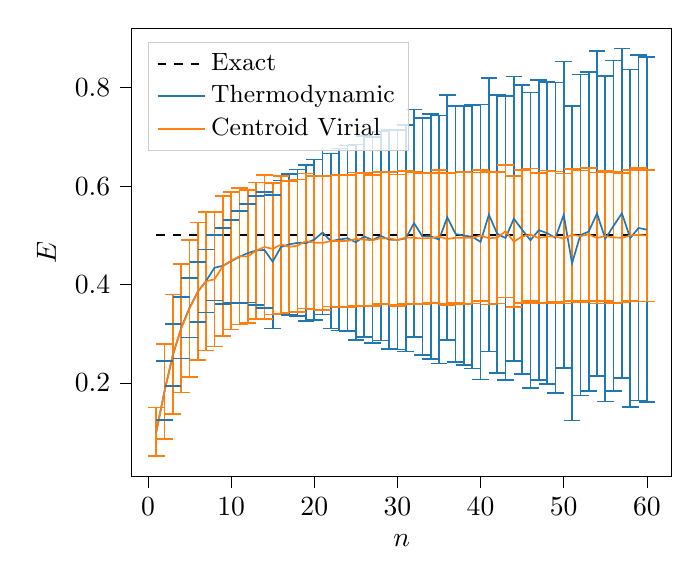
\begin{tikzpicture}

\definecolor{darkgray176}{RGB}{176,176,176}
\definecolor{darkorange25512714}{RGB}{255,127,14}
\definecolor{lightgray204}{RGB}{204,204,204}
\definecolor{steelblue31119180}{RGB}{31,119,180}

\begin{axis}[
legend cell align={left},
legend style={
  fill opacity=0.8,
  draw opacity=1,
  text opacity=1,
  at={(0.03,0.97)},
  anchor=north west,
  draw=lightgray204
},
tick align=outside,
tick pos=left,
x grid style={darkgray176},
xlabel={\(\displaystyle n\)},
xmin=-1.95, xmax=62.95,
xtick style={color=black},
y grid style={darkgray176},
ylabel={\(\displaystyle E\)},
ymin=0.00985367642610356, ymax=0.920718110499366,
ytick style={color=black},
legend entries={\small Exact,,,,,\small Thermodynamic,\small Centroid Virial},
]
\addplot [semithick, black, dashed]
table {%
1 0.50004540199101
60 0.50004540199101
};

\path [draw=steelblue31119180, semithick]
(axis cs:1,0.0512566052476155)
--(axis cs:1,0.150361644878232);

\path [draw=steelblue31119180, semithick]
(axis cs:2,0.124237266806461)
--(axis cs:2,0.24468435113687);

\path [draw=steelblue31119180, semithick]
(axis cs:3,0.19350175551363)
--(axis cs:3,0.319790856706941);

\path [draw=steelblue31119180, semithick]
(axis cs:4,0.249416997423427)
--(axis cs:4,0.374766263491673);

\path [draw=steelblue31119180, semithick]
(axis cs:5,0.292023715410442)
--(axis cs:5,0.413820112852047);

\path [draw=steelblue31119180, semithick]
(axis cs:6,0.324279293107666)
--(axis cs:6,0.44640955402721);

\path [draw=steelblue31119180, semithick]
(axis cs:7,0.343427611891579)
--(axis cs:7,0.471468021602742);

\path [draw=steelblue31119180, semithick]
(axis cs:8,0.367857960482131)
--(axis cs:8,0.500565575729486);

\path [draw=steelblue31119180, semithick]
(axis cs:9,0.360955550039732)
--(axis cs:9,0.514860353268616);

\path [draw=steelblue31119180, semithick]
(axis cs:10,0.362940944045004)
--(axis cs:10,0.531670205308182);

\path [draw=steelblue31119180, semithick]
(axis cs:11,0.362788354813513)
--(axis cs:11,0.549651033653193);

\path [draw=steelblue31119180, semithick]
(axis cs:12,0.363333465287984)
--(axis cs:12,0.564230295876903);

\path [draw=steelblue31119180, semithick]
(axis cs:13,0.358044876121361)
--(axis cs:13,0.579955401006553);

\path [draw=steelblue31119180, semithick]
(axis cs:14,0.352455765674314)
--(axis cs:14,0.58813441799208);

\path [draw=steelblue31119180, semithick]
(axis cs:15,0.310405129316881)
--(axis cs:15,0.582453488549705);

\path [draw=steelblue31119180, semithick]
(axis cs:16,0.341224204045176)
--(axis cs:16,0.611451131852651);

\path [draw=steelblue31119180, semithick]
(axis cs:17,0.338571483526223)
--(axis cs:17,0.624764583709684);

\path [draw=steelblue31119180, semithick]
(axis cs:18,0.335741404206791)
--(axis cs:18,0.633513497376222);

\path [draw=steelblue31119180, semithick]
(axis cs:19,0.32549929242973)
--(axis cs:19,0.642565088720023);

\path [draw=steelblue31119180, semithick]
(axis cs:20,0.328438437532902)
--(axis cs:20,0.654243740078346);

\path [draw=steelblue31119180, semithick]
(axis cs:21,0.33894701070065)
--(axis cs:21,0.672310198402497);

\path [draw=steelblue31119180, semithick]
(axis cs:22,0.310354186855867)
--(axis cs:22,0.666106762576854);

\path [draw=steelblue31119180, semithick]
(axis cs:23,0.306608789483003)
--(axis cs:23,0.676255739058717);

\path [draw=steelblue31119180, semithick]
(axis cs:24,0.305039889872913)
--(axis cs:24,0.682724188247641);

\path [draw=steelblue31119180, semithick]
(axis cs:25,0.287778133191332)
--(axis cs:25,0.6841905294068);

\path [draw=steelblue31119180, semithick]
(axis cs:26,0.293829005932844)
--(axis cs:26,0.701308213575541);

\path [draw=steelblue31119180, semithick]
(axis cs:27,0.280707613978325)
--(axis cs:27,0.700376010762016);

\path [draw=steelblue31119180, semithick]
(axis cs:28,0.286603412750338)
--(axis cs:28,0.710774388151236);

\path [draw=steelblue31119180, semithick]
(axis cs:29,0.268521557781578)
--(axis cs:29,0.714153755236597);

\path [draw=steelblue31119180, semithick]
(axis cs:30,0.267650320930231)
--(axis cs:30,0.713344407946041);

\path [draw=steelblue31119180, semithick]
(axis cs:31,0.263768826727663)
--(axis cs:31,0.72377533120979);

\path [draw=steelblue31119180, semithick]
(axis cs:32,0.29372514129932)
--(axis cs:32,0.755765975790672);

\path [draw=steelblue31119180, semithick]
(axis cs:33,0.256848758400715)
--(axis cs:33,0.738890106992184);

\path [draw=steelblue31119180, semithick]
(axis cs:34,0.248882966137649)
--(axis cs:34,0.747059063267314);

\path [draw=steelblue31119180, semithick]
(axis cs:35,0.239447383672488)
--(axis cs:35,0.743304191150986);

\path [draw=steelblue31119180, semithick]
(axis cs:36,0.287567922066669)
--(axis cs:36,0.785530942752071);

\path [draw=steelblue31119180, semithick]
(axis cs:37,0.243115423517044)
--(axis cs:37,0.762033013016613);

\path [draw=steelblue31119180, semithick]
(axis cs:38,0.236682064579175)
--(axis cs:38,0.761929270324992);

\path [draw=steelblue31119180, semithick]
(axis cs:39,0.229553054890202)
--(axis cs:39,0.764570503777587);

\path [draw=steelblue31119180, semithick]
(axis cs:40,0.207379991743943)
--(axis cs:40,0.765814932230782);

\path [draw=steelblue31119180, semithick]
(axis cs:41,0.264169670539953)
--(axis cs:41,0.819812792722688);

\path [draw=steelblue31119180, semithick]
(axis cs:42,0.220728403871344)
--(axis cs:42,0.785598197401665);

\path [draw=steelblue31119180, semithick]
(axis cs:43,0.205662485448271)
--(axis cs:43,0.783279258734133);

\path [draw=steelblue31119180, semithick]
(axis cs:44,0.245082840950098)
--(axis cs:44,0.822485721939277);

\path [draw=steelblue31119180, semithick]
(axis cs:45,0.217759115373799)
--(axis cs:45,0.804829690345888);

\path [draw=steelblue31119180, semithick]
(axis cs:46,0.189746195798166)
--(axis cs:46,0.790093234121875);

\path [draw=steelblue31119180, semithick]
(axis cs:47,0.205727040354122)
--(axis cs:47,0.814982667023599);

\path [draw=steelblue31119180, semithick]
(axis cs:48,0.197329138265573)
--(axis cs:48,0.811496514068311);

\path [draw=steelblue31119180, semithick]
(axis cs:49,0.178970897946345)
--(axis cs:49,0.810640716417495);

\path [draw=steelblue31119180, semithick]
(axis cs:50,0.230255344784278)
--(axis cs:50,0.852964103408094);

\path [draw=steelblue31119180, semithick]
(axis cs:51,0.123616678482179)
--(axis cs:51,0.762697530565664);

\path [draw=steelblue31119180, semithick]
(axis cs:52,0.174480365792205)
--(axis cs:52,0.826375290522613);

\path [draw=steelblue31119180, semithick]
(axis cs:53,0.183043627737482)
--(axis cs:53,0.831846694042412);

\path [draw=steelblue31119180, semithick]
(axis cs:54,0.214146231862649)
--(axis cs:54,0.874509879292435);

\path [draw=steelblue31119180, semithick]
(axis cs:55,0.162194808642373)
--(axis cs:55,0.823744720345098);

\path [draw=steelblue31119180, semithick]
(axis cs:56,0.183744134211075)
--(axis cs:56,0.855058326824435);

\path [draw=steelblue31119180, semithick]
(axis cs:57,0.210129643477892)
--(axis cs:57,0.879315181677854);

\path [draw=steelblue31119180, semithick]
(axis cs:58,0.151735890363417)
--(axis cs:58,0.83691911938825);

\path [draw=steelblue31119180, semithick]
(axis cs:59,0.164197314037449)
--(axis cs:59,0.86570555892238);

\path [draw=steelblue31119180, semithick]
(axis cs:60,0.160929442551088)
--(axis cs:60,0.861875209415569);

\addplot [semithick, steelblue31119180, mark=-, mark size=3, mark options={solid}, only marks]
table {%
1 0.0512566052476155
2 0.124237266806461
3 0.19350175551363
4 0.249416997423427
5 0.292023715410442
6 0.324279293107666
7 0.343427611891579
8 0.367857960482131
9 0.360955550039732
10 0.362940944045004
11 0.362788354813513
12 0.363333465287984
13 0.358044876121361
14 0.352455765674314
15 0.310405129316881
16 0.341224204045176
17 0.338571483526223
18 0.335741404206791
19 0.32549929242973
20 0.328438437532902
21 0.33894701070065
22 0.310354186855867
23 0.306608789483003
24 0.305039889872913
25 0.287778133191332
26 0.293829005932844
27 0.280707613978325
28 0.286603412750338
29 0.268521557781578
30 0.267650320930231
31 0.263768826727663
32 0.29372514129932
33 0.256848758400715
34 0.248882966137649
35 0.239447383672488
36 0.287567922066669
37 0.243115423517044
38 0.236682064579175
39 0.229553054890202
40 0.207379991743943
41 0.264169670539953
42 0.220728403871344
43 0.205662485448271
44 0.245082840950098
45 0.217759115373799
46 0.189746195798166
47 0.205727040354122
48 0.197329138265573
49 0.178970897946345
50 0.230255344784278
51 0.123616678482179
52 0.174480365792205
53 0.183043627737482
54 0.214146231862649
55 0.162194808642373
56 0.183744134211075
57 0.210129643477892
58 0.151735890363417
59 0.164197314037449
60 0.160929442551088
};

\addplot [semithick, steelblue31119180, mark=-, mark size=3, mark options={solid}, only marks]
table {%
1 0.150361644878232
2 0.24468435113687
3 0.319790856706941
4 0.374766263491673
5 0.413820112852047
6 0.44640955402721
7 0.471468021602742
8 0.500565575729486
9 0.514860353268616
10 0.531670205308182
11 0.549651033653193
12 0.564230295876903
13 0.579955401006553
14 0.58813441799208
15 0.582453488549705
16 0.611451131852651
17 0.624764583709684
18 0.633513497376222
19 0.642565088720023
20 0.654243740078346
21 0.672310198402497
22 0.666106762576854
23 0.676255739058717
24 0.682724188247641
25 0.6841905294068
26 0.701308213575541
27 0.700376010762016
28 0.710774388151236
29 0.714153755236597
30 0.713344407946041
31 0.72377533120979
32 0.755765975790672
33 0.738890106992184
34 0.747059063267314
35 0.743304191150986
36 0.785530942752071
37 0.762033013016613
38 0.761929270324992
39 0.764570503777587
40 0.765814932230782
41 0.819812792722688
42 0.785598197401665
43 0.783279258734133
44 0.822485721939277
45 0.804829690345888
46 0.790093234121875
47 0.814982667023599
48 0.811496514068311
49 0.810640716417495
50 0.852964103408094
51 0.762697530565664
52 0.826375290522613
53 0.831846694042412
54 0.874509879292435
55 0.823744720345098
56 0.855058326824435
57 0.879315181677854
58 0.83691911938825
59 0.86570555892238
60 0.861875209415569
};

\path [draw=darkorange25512714, semithick]
(axis cs:1,0.0512566052476155)
--(axis cs:1,0.150361644878232);

\path [draw=darkorange25512714, semithick]
(axis cs:2,0.0866744161675931)
--(axis cs:2,0.279625555456749);

\path [draw=darkorange25512714, semithick]
(axis cs:3,0.136940491864086)
--(axis cs:3,0.379491607238542);

\path [draw=darkorange25512714, semithick]
(axis cs:4,0.180291667967983)
--(axis cs:4,0.441349672314435);

\path [draw=darkorange25512714, semithick]
(axis cs:5,0.212668942698273)
--(axis cs:5,0.489820501965271);

\path [draw=darkorange25512714, semithick]
(axis cs:6,0.246217094840295)
--(axis cs:6,0.52623438820376);

\path [draw=darkorange25512714, semithick]
(axis cs:7,0.266007695652659)
--(axis cs:7,0.547498746483928);

\path [draw=darkorange25512714, semithick]
(axis cs:8,0.273767844295365)
--(axis cs:8,0.547484794685045);

\path [draw=darkorange25512714, semithick]
(axis cs:9,0.295409263680663)
--(axis cs:9,0.579362340500812);

\path [draw=darkorange25512714, semithick]
(axis cs:10,0.308333991510197)
--(axis cs:10,0.588306825652258);

\path [draw=darkorange25512714, semithick]
(axis cs:11,0.318867717028158)
--(axis cs:11,0.596008693203401);

\path [draw=darkorange25512714, semithick]
(axis cs:12,0.321274605677066)
--(axis cs:12,0.592681223766939);

\path [draw=darkorange25512714, semithick]
(axis cs:13,0.330363337023986)
--(axis cs:13,0.607117477099351);

\path [draw=darkorange25512714, semithick]
(axis cs:14,0.329703342429675)
--(axis cs:14,0.62277259682354);

\path [draw=darkorange25512714, semithick]
(axis cs:15,0.338843135954417)
--(axis cs:15,0.606208328557809);

\path [draw=darkorange25512714, semithick]
(axis cs:16,0.341392432563182)
--(axis cs:16,0.621009629777026);

\path [draw=darkorange25512714, semithick]
(axis cs:17,0.342902345893601)
--(axis cs:17,0.610283037196728);

\path [draw=darkorange25512714, semithick]
(axis cs:18,0.34430953327113)
--(axis cs:18,0.613362595365798);

\path [draw=darkorange25512714, semithick]
(axis cs:19,0.35131205489719)
--(axis cs:19,0.625278168366129);

\path [draw=darkorange25512714, semithick]
(axis cs:20,0.349083766614378)
--(axis cs:20,0.62081198041454);

\path [draw=darkorange25512714, semithick]
(axis cs:21,0.348583577376329)
--(axis cs:21,0.620713201653813);

\path [draw=darkorange25512714, semithick]
(axis cs:22,0.355306496907812)
--(axis cs:22,0.621287664516584);

\path [draw=darkorange25512714, semithick]
(axis cs:23,0.354896497269853)
--(axis cs:23,0.621849398020325);

\path [draw=darkorange25512714, semithick]
(axis cs:24,0.354289621213389)
--(axis cs:24,0.623045722259879);

\path [draw=darkorange25512714, semithick]
(axis cs:25,0.357389431473731)
--(axis cs:25,0.627621864236831);

\path [draw=darkorange25512714, semithick]
(axis cs:26,0.355953035375493)
--(axis cs:26,0.626449945246168);

\path [draw=darkorange25512714, semithick]
(axis cs:27,0.356975920855537)
--(axis cs:27,0.622748840529471);

\path [draw=darkorange25512714, semithick]
(axis cs:28,0.360118335498707)
--(axis cs:28,0.628343065476657);

\path [draw=darkorange25512714, semithick]
(axis cs:29,0.359440059944409)
--(axis cs:29,0.628599949344922);

\path [draw=darkorange25512714, semithick]
(axis cs:30,0.35679788032375)
--(axis cs:30,0.623552577497206);

\path [draw=darkorange25512714, semithick]
(axis cs:31,0.360518634049624)
--(axis cs:31,0.630701612653681);

\path [draw=darkorange25512714, semithick]
(axis cs:32,0.360799480863554)
--(axis cs:32,0.628685465780561);

\path [draw=darkorange25512714, semithick]
(axis cs:33,0.360160888602783)
--(axis cs:33,0.626951665224133);

\path [draw=darkorange25512714, semithick]
(axis cs:34,0.362072796397728)
--(axis cs:34,0.626771828843405);

\path [draw=darkorange25512714, semithick]
(axis cs:35,0.361266128452568)
--(axis cs:35,0.632828239471349);

\path [draw=darkorange25512714, semithick]
(axis cs:36,0.358594939958791)
--(axis cs:36,0.626858032843862);

\path [draw=darkorange25512714, semithick]
(axis cs:37,0.362125816127054)
--(axis cs:37,0.627693679852222);

\path [draw=darkorange25512714, semithick]
(axis cs:38,0.360159100255577)
--(axis cs:38,0.629842187813911);

\path [draw=darkorange25512714, semithick]
(axis cs:39,0.361654477050002)
--(axis cs:39,0.627877496892953);

\path [draw=darkorange25512714, semithick]
(axis cs:40,0.366410425887438)
--(axis cs:40,0.632727673377995);

\path [draw=darkorange25512714, semithick]
(axis cs:41,0.359695011066873)
--(axis cs:41,0.628349105628929);

\path [draw=darkorange25512714, semithick]
(axis cs:42,0.361168046020572)
--(axis cs:42,0.629160041816989);

\path [draw=darkorange25512714, semithick]
(axis cs:43,0.373774440267227)
--(axis cs:43,0.64276396767651);

\path [draw=darkorange25512714, semithick]
(axis cs:44,0.353829059546958)
--(axis cs:44,0.620560287516075);

\path [draw=darkorange25512714, semithick]
(axis cs:45,0.363097981505745)
--(axis cs:45,0.632261371229761);

\path [draw=darkorange25512714, semithick]
(axis cs:46,0.366736847991824)
--(axis cs:46,0.635848212848707);

\path [draw=darkorange25512714, semithick]
(axis cs:47,0.362225548003136)
--(axis cs:47,0.626661042571855);

\path [draw=darkorange25512714, semithick]
(axis cs:48,0.363106780580795)
--(axis cs:48,0.631712468130891);

\path [draw=darkorange25512714, semithick]
(axis cs:49,0.364872331022633)
--(axis cs:49,0.629852671658989);

\path [draw=darkorange25512714, semithick]
(axis cs:50,0.361153989628477)
--(axis cs:50,0.625252221993808);

\path [draw=darkorange25512714, semithick]
(axis cs:51,0.367165122318732)
--(axis cs:51,0.635270769255034);

\path [draw=darkorange25512714, semithick]
(axis cs:52,0.364612992788832)
--(axis cs:52,0.631763845175859);

\path [draw=darkorange25512714, semithick]
(axis cs:53,0.367117616539792)
--(axis cs:53,0.636925997619656);

\path [draw=darkorange25512714, semithick]
(axis cs:54,0.361521059145079)
--(axis cs:54,0.627539744058306);

\path [draw=darkorange25512714, semithick]
(axis cs:55,0.365982239769132)
--(axis cs:55,0.630693073817261);

\path [draw=darkorange25512714, semithick]
(axis cs:56,0.362555754968832)
--(axis cs:56,0.628497132274725);

\path [draw=darkorange25512714, semithick]
(axis cs:57,0.363620051415977)
--(axis cs:57,0.626387517867149);

\path [draw=darkorange25512714, semithick]
(axis cs:58,0.366883384617054)
--(axis cs:58,0.632110750265377);

\path [draw=darkorange25512714, semithick]
(axis cs:59,0.365704249948489)
--(axis cs:59,0.63615089379198);

\path [draw=darkorange25512714, semithick]
(axis cs:60,0.365830172876832)
--(axis cs:60,0.632972388598584);

\addplot [semithick, darkorange25512714, mark=-, mark size=3, mark options={solid}, only marks]
table {%
1 0.0512566052476155
2 0.0866744161675931
3 0.136940491864086
4 0.180291667967983
5 0.212668942698273
6 0.246217094840295
7 0.266007695652659
8 0.273767844295365
9 0.295409263680663
10 0.308333991510197
11 0.318867717028158
12 0.321274605677066
13 0.330363337023986
14 0.329703342429675
15 0.338843135954417
16 0.341392432563182
17 0.342902345893601
18 0.34430953327113
19 0.35131205489719
20 0.349083766614378
21 0.348583577376329
22 0.355306496907812
23 0.354896497269853
24 0.354289621213389
25 0.357389431473731
26 0.355953035375493
27 0.356975920855537
28 0.360118335498707
29 0.359440059944409
30 0.35679788032375
31 0.360518634049624
32 0.360799480863554
33 0.360160888602783
34 0.362072796397728
35 0.361266128452568
36 0.358594939958791
37 0.362125816127054
38 0.360159100255577
39 0.361654477050002
40 0.366410425887438
41 0.359695011066873
42 0.361168046020572
43 0.373774440267227
44 0.353829059546958
45 0.363097981505745
46 0.366736847991824
47 0.362225548003136
48 0.363106780580795
49 0.364872331022633
50 0.361153989628477
51 0.367165122318732
52 0.364612992788832
53 0.367117616539792
54 0.361521059145079
55 0.365982239769132
56 0.362555754968832
57 0.363620051415977
58 0.366883384617054
59 0.365704249948489
60 0.365830172876832
};

\addplot [semithick, darkorange25512714, mark=-, mark size=3, mark options={solid}, only marks]
table {%
1 0.150361644878232
2 0.279625555456749
3 0.379491607238542
4 0.441349672314435
5 0.489820501965271
6 0.52623438820376
7 0.547498746483928
8 0.547484794685045
9 0.579362340500812
10 0.588306825652258
11 0.596008693203401
12 0.592681223766939
13 0.607117477099351
14 0.62277259682354
15 0.606208328557809
16 0.621009629777026
17 0.610283037196728
18 0.613362595365798
19 0.625278168366129
20 0.62081198041454
21 0.620713201653813
22 0.621287664516584
23 0.621849398020325
24 0.623045722259879
25 0.627621864236831
26 0.626449945246168
27 0.622748840529471
28 0.628343065476657
29 0.628599949344922
30 0.623552577497206
31 0.630701612653681
32 0.628685465780561
33 0.626951665224133
34 0.626771828843405
35 0.632828239471349
36 0.626858032843862
37 0.627693679852222
38 0.629842187813911
39 0.627877496892953
40 0.632727673377995
41 0.628349105628929
42 0.629160041816989
43 0.64276396767651
44 0.620560287516075
45 0.632261371229761
46 0.635848212848707
47 0.626661042571855
48 0.631712468130891
49 0.629852671658989
50 0.625252221993808
51 0.635270769255034
52 0.631763845175859
53 0.636925997619656
54 0.627539744058306
55 0.630693073817261
56 0.628497132274725
57 0.626387517867149
58 0.632110750265377
59 0.63615089379198
60 0.632972388598584
};

\addplot [semithick, steelblue31119180]
table {%
1 0.100809125062924
2 0.184460808971665
3 0.256646306110286
4 0.31209163045755
5 0.352921914131245
6 0.385344423567438
7 0.40744781674716
8 0.434211768105809
9 0.437907951654174
10 0.447305574676593
11 0.456219694233353
12 0.463781880582444
13 0.469000138563957
14 0.470295091833197
15 0.446429308933293
16 0.476337667948913
17 0.481668033617953
18 0.484627450791507
19 0.484032190574877
20 0.491341088805624
21 0.505628604551573
22 0.48823047471636
23 0.49143226427086
24 0.493882039060277
25 0.485984331299066
26 0.497568609754192
27 0.490541812370171
28 0.498688900450787
29 0.491337656509088
30 0.490497364438136
31 0.493772078968726
32 0.524745558544996
33 0.497869432696449
34 0.497971014702482
35 0.491375787411737
36 0.53654943240937
37 0.502574218266829
38 0.499305667452083
39 0.497061779333895
40 0.486597461987363
41 0.54199123163132
42 0.503163300636505
43 0.494470872091202
44 0.533784281444687
45 0.511294402859843
46 0.489919714960021
47 0.51035485368886
48 0.504412826166942
49 0.49480580718192
50 0.541609724096186
51 0.443157104523922
52 0.500427828157409
53 0.507445160889947
54 0.544328055577542
55 0.492969764493736
56 0.519401230517755
57 0.544722412577873
58 0.494327504875834
59 0.514951436479915
60 0.511402325983329
};

\addplot [semithick, darkorange25512714]
table {%
1 0.100809125062924
2 0.183149985812171
3 0.258216049551314
4 0.310820670141209
5 0.351244722331772
6 0.386225741522027
7 0.406753221068294
8 0.410626319490205
9 0.437385802090737
10 0.448320408581227
11 0.457438205115779
12 0.456977914722003
13 0.468740407061669
14 0.476237969626608
15 0.472525732256113
16 0.481201031170104
17 0.476592691545165
18 0.478836064318464
19 0.48829511163166
20 0.484947873514459
21 0.484648389515071
22 0.488297080712198
23 0.488372947645089
24 0.488667671736634
25 0.492505647855281
26 0.49120149031083
27 0.489862380692504
28 0.494230700487682
29 0.494020004644665
30 0.490175228910478
31 0.495610123351653
32 0.494742473322057
33 0.493556276913458
34 0.494422312620566
35 0.497047183961958
36 0.492726486401326
37 0.494909747989638
38 0.495000644034744
39 0.494765986971478
40 0.499569049632716
41 0.494022058347901
42 0.49516404391878
43 0.508269203971869
44 0.487194673531516
45 0.497679676367753
46 0.501292530420265
47 0.494443295287496
48 0.497409624355843
49 0.497362501340811
50 0.493203105811142
51 0.501217945786883
52 0.498188418982346
53 0.502021807079724
54 0.494530401601693
55 0.498337656793196
56 0.495526443621778
57 0.495003784641563
58 0.499497067441216
59 0.500927571870235
60 0.499401280737708
};

\end{axis}

\end{tikzpicture}

        \caption{Average energies of a harmonic oscillator with \(\beta\hbar\omega=10\), sampled with 20000 runs using the two estimators. The error bars are the standard deviation of the energies.}
    \end{figure}
    In the example above, both thermodynamic energy estimator and centroid virial estimator converges to the exact \(\eval{E}\) as \(n\to\infty\). However, the standard deviation of the thermodynamic estimator grows asymptotically as \(\sqrt{n}\), so the required number of sample would increase linearly with \(n\) to keep the standard error in the mean constant. By contrast, the standard deviation of the centroid virial estimator is asymmetrically constant of \(n\). 

    \newpage
    \section{Propagating the Ring Polymer Dynamics}
    \subsection{Integrating the Equations of Motion}
    In the previous section, we have established that to sample the equilibrium thermal average of some quantum system, we can instead propagate the dynamics of a classical ring polymer system and sample the thermal average of the corresponding classical estimator. This is known as the \textit{path integral molecular dynamics} (PIMD).

    Given a classical Hamiltonian \(H(\vb{p},\vb{q})\) with initial conditions \(\vb{p}(0)=\vb{p}_0\), \(\vb{q}(0)=\vb{q}_0\), the evolution of the system is governed deterministically by the Hamilton's equation
    \begin{align}
        \dot{\vb{p}}=-\pdv{H}{\vb{q}} \\
        \dot{\vb{q}}=+\pdv{H}{\vb{p}}\,.
    \end{align}
    For our Hamiltonian \(H=\frac{\vb{p}^2}{2m}+V(\vb{q})\), this is
    \begin{align}
        \dot{\vb{p}}=-\pdv{V}{\vb{q}} \\
        \dot{\vb{q}}=+\frac{\vb{p}}{m}
    \end{align}
    as one would expect from Newton's second law.

    These are a set of differential equations, and to work out the trajectory, we need to integrate these equations of motion. The most common way to do this is to use the velocity Verlet algorithm (see my notes on NST Part II C8: \textit{Computer Simulation Methods}), in which the following steps are carried out iteratively to propagate the dynamics:
    \begin{align}
        \vb{p}_{n+\frac{1}{2}}&=\vb{p}_{n}-\frac{\delta t}{2}\pdv{V}{\vb{q}}(\vb{q}_{n})  \\
        \vb{q}_{n+1}&=\vb{q}+\delta t\frac{\vb{p}_{n+\frac{1}{2}}}{m} \\
        \vb{p}_{n+1}&=\vb{p}_{n+\frac{1}{2}}-\frac{\delta t}{2}\pdv{V}{\vb{q}}(\vb{q}_{n+1})\,.
    \end{align}
    This propagates the momenta under \(V\) by half a time step, propagates the coordinates by a full time step, and then propagate the momenta by another time step, corresponding to symmetrically splitting the time evolution operator by
    \begin{equation}
        \ee^{-\mathcal{L}\delta t}\simeq \ee^{-\mathcal{L}_V\delta t/2}\ee^{-\mathcal{L}_T \delta t}\ee^{-\mathcal{L}_V/2}\,.
    \end{equation}
    This is accurate to \(O(\delta t^3)\) for each time step (\(O(\delta t^2)\) globally), and is better than propagating the coordinates and momenta by a full time step simultaneously, which is known as the Euler's algorithm and is accurate to \(O(\delta t^2)\) each step and \(O(\delta t)\) globally.

    For path integral molecular dynamics, we can of course directly use the standard velocity Verlet algorithm with Hamiltonian
    \begin{equation}
        H_n(\vb{p},\vb{q})=\frac{\vb{p}^2}{2m}+V(\vb{q})\,,
    \end{equation}
    where
    \begin{equation}
        V(\vb{q})=\sum_{j=1}^{n}\left[\frac{1}{2}m\omega_n^2(q_j-q_{j+1})^2+V(q_j)\right]\,,
    \end{equation}
    to propagate the dynamics. However, the harmonic springs between the beads are stiff, especially with large \(n\) (\(\omega_n=n/\beta\hbar\)). This requires a very small time step for us to propagate the internal vibrations of the ring polymer beads accurately. (Usually a time step of \(1/20\) of the shortest characteristic vibrational time scale of the system is safe.)

    Luckily, we know how to solve the vibrational motions of systems connected by harmonic springs exactly! We can break them down to normal modes and propagate these internal normal modes exactly. (See NST Part II C8: \textit{Further Quantum Mechanics} or NST Part IB Mathematical Methods.) We break down the Hamiltonian as
    \begin{equation}
        H_{n}(\vb{p},\vb{q})=H_{n,0}(\vb{p},\vb{q})+V_{n}(\vb{q})\,,
    \end{equation}
    where
    \begin{equation}
        H_{n, 0}=\sum_{j=1}^{n}\left[\frac{p_j^2}{2m}+\frac{1}{2}m\omega_n^2(q_j-q_{j+1})^2\right]
    \end{equation}
    is the free ring polymer Hamiltonian without the external potential and
    \begin{equation}
        V_n(\vb{q})=\sum_{j=1}^{n}V(q_j)
    \end{equation}
    is the external potential. Since the potential of the free ring polymer Hamiltonian \(H_0(\vb{p},\vb{q})\) is harmonic, it can be diagonalised with a normal mode transformation
    \begin{equation}\label{normal_mode_transformation}
        \begin{cases}
            \tilde{p}_k=\sum_{j=1}^{n}p_jC_{jk}\\
            \tilde{q}_k=\sum_{j=1}^{n}q_jC_{jk}\,,
        \end{cases}
    \end{equation}
    where
    \begin{equation}
        C_{jk}=\begin{cases}
            \sqrt{1/n} & k=0 \\
            \sqrt{2/n}\cos(2\pi jk/n) & 1\le k\le n/2 -1 \\
            \sqrt{1/2} (-1)^j & k=n/2 \\
            \sqrt{2/n}\sin(2\pi jk/n) &n/2+1 \le k \le n\,,
        \end{cases}
    \end{equation}
    giving
    \begin{equation}
        H_0(\tilde{\vb{p}},\tilde{\vb{q}})=\sum_{k=0}^{n-1}\left[\frac{\tilde{p}_k^2}{2m}+\frac{1}{2}m\omega_k^2\tilde{q}_k^2\right]
    \end{equation}
    with
    \begin{equation}
        \omega_k=2\omega_n\sin\left(\frac{k\pi}{n}\right)\,.
    \end{equation}
    Notice that we have shifted the range of indices from \(1\le j\le n\) to \(0\le k\le n-1\). You should be familiar with this because \(C_{jk}\) and \(\omega_k^2\) are actually exactly the H\"{u}ckel molecular orbital coefficients and the orbital energies of a cyclic polyene. This is because the H\"{u}ckel matrix of a cyclic polyene and the potential energy matrix of a ring polymer are exactly the same:
    \begin{equation}
        \mathsf{H}_{\text{polyene}}=\begin{pmatrix}
            \alpha & \beta & 0 & \cdots & \beta \\
            \beta & \alpha & \beta & \cdots & 0 \\
            0 & \beta & \alpha & \cdots & 0 \\
            \vdots & \vdots & \vdots & \ddots & \vdots \\
            \beta & 0 & 0 & \cdots & \alpha
        \end{pmatrix}\quad\stackrel{\alpha=2,\beta=-1}{\longleftrightarrow}\quad\mathsf{V}=\begin{pmatrix}
            2 & -1 & 0 & \cdots & -1 \\
            -1 & 2 & -1 & \cdots & 0 \\
            0 & -1 & 2 & \cdots & 0 \\
            \vdots & \vdots & \vdots & \ddots & \vdots \\
            -1 & 0 & 0 & \cdots & 2
        \end{pmatrix}
    \end{equation}
    such that \(\sum_{j=1}^{n}(q_j-q_{j+1})^2=\vb{q}\tp \mathsf{V}\vb{q}\). Moreover, the normal mode transformation (\ref{normal_mode_transformation}) is exactly the discrete Fourier transform, which can be efficiently carried out using the Fast Fourier Transform (FFT) algorithm with a scaling no larger than \(O(n\log n)\).

    In the normal mode coordinates, the Hamiltonian \(H_{0,n}\) is broken down into \(n\) independent harmonic oscillators, each evolving sinusoidally
    \begin{equation}
        \begin{cases}
            \tilde{q}_k=A_k\sin(\omega_k t) + B_k\cos(\omega_k t) \\
            \tilde{p}_k=mA_k\omega_k\cos(\omega_k t) - mB_k\omega_k\cos(\omega_k t)\,.
        \end{cases}
    \end{equation} 
    
    To overall idea is therefore breaking down the ring polymer evolution by
    \begin{equation}
        \ee^{-\mathcal{L}\delta t}=\ee^{-\mathcal{L}_V\delta /2}\ee^{-\mathcal{L}_0\delta t}\ee^{-\mathcal{L}_V\delta t/2}\,,
    \end{equation}
    i.e. evolve the momenta by the external potential for half a time step, transform into the normal mode coordinates, evolve the coordinates and momenta by the internal ring normal modes for a full time step, revert back to the real coordinates, and finally evolve the momenta by the external potential for half a time step. The detailed algorithm is
    \begin{align}
        \vb{p}'&=\vb{p}_n-\frac{\delta t}{2}\dv{V}{\vb{q}}(\vb{q}_n)\\
        \tilde{\vb{p}}'&=\mathsf{C}\tp\vb{p}'\\
        \tilde{\vb{q}}'&=\mathsf{C}\tp\vb{q}_n\\
        \begin{pmatrix}
            \tilde{p}_k'' \\
            \tilde{q}_k''
        \end{pmatrix}&=\begin{pmatrix}
            \cos\omega_k\delta t & -m\omega_k \sin\omega_k\delta t \\
            \frac{1}{m\omega_k}\sin\omega_k\delta t & \cos\omega_k\delta t
        \end{pmatrix}\begin{pmatrix}
            \tilde{p}_k' \\
            \tilde{q}_k'
        \end{pmatrix} \\
        \vb{p}''&=\mathsf{C}\tilde{\vb{p}}''\\
        \vb{q}_{n+1}&=\mathsf{C}\tilde{\vb{q}}''\\
        \vb{p}_{n+1}&=\vb{p}''-\frac{\delta t}{2}\dv{V}{\vb{q}}(\vb{q}_{n+1})
    \end{align}

    \subsection{Sampling in Canonical Ensemble}
    The above algorithm well propagates the dynamics of the ring polymer in a microcanonical ensemble, but we can't use them to calculate canonical thermal averages because
    \begin{itemize}
        \item The above algorithm rigorously conserves the energy \(H_n\). Instead in a canonical ensemble with constant energy, the phase space should be sampled with all possible \(H_n\) weighted by their Boltzmann factors.
        \item It is far from ergodic. If the external potential is harmonic, then the whole \(H_n\) is diagonal in the normal mode representation and hence there is no energy flow between the normal modes. If the external potential is instead mildly anharmonic, then the energy exchanges between modes very slowly. It is therefore not even possible to fully sample the microcanonical constant energy hypersurface in the phase space ergodically within the typical timescale of a simulation.
    \end{itemize}

    Therefore to meaningfully work out a thermal average, we need to attach a thermostat to our ring polymer system. Here we will briefly introduce the path integral Langevin equation (PILE) thermostat.

    \subsubsection{The Path Integral Langevin Equation Thermostat}
    The PILE thermostat attaches a separate Langevin thermostat to each internal mode of the free ring polymer, so that the free polymer would evolve by
    \begin{align}
        \dv{}{t}\tilde{q}_k&=\frac{\tilde{p}_k}{m} \\
        \dv{}{t}\tilde{p}_k&=-m\omega_k^2\tilde{q}_k-\gamma_k\tilde{p}_k+\sqrt{\frac{2m\gamma_k}{\beta_n}}\xi_k(t)\,,\label{Langevin_momentum}
    \end{align}
    where \(\gamma_k(t)\) represents an uncorrelated, Gaussian-distributed random form with unit variance and zero mean:
    \begin{equation}
        \eval{\xi_k(t)}=0\qquad \eval{\xi_k(0)\xi_k(t)}=\delta(t)\,,
    \end{equation}
    and the \textit{friction coefficients} \(\gamma_k\) governs the rate at which the velocities are thermalised. The first term in (\ref{Langevin_momentum}) is the free evolution of a microcanonical harmonic oscillator, and the two extra terms are from the Langevin thermostat. Their origins are explained in NST Part II B7: \textit{Statistical Mechanics}.

    The PILE thermostat uses the propagator
    \begin{equation}
        \ee^{-\mathcal{L}_\gamma \delta t/2}\ee^{-\mathcal{L}_V\delta t/2}\ee^{-\mathcal{L}_0\delta t}\ee^{-\mathcal{L}_V\delta t/2}\ee^{-\mathcal{L}_\gamma\delta t/2}\,,
    \end{equation}
    where the extra thermostatting steps (\(\ee^{-\mathcal{L}_\gamma\delta t/2}\)) implements the last two extra terms in (\ref{Langevin_momentum}). They are implemented by
    \begin{align}
        \tilde{p}_k &= \sum_{j=1}^{n} p_j C_{jk} \\
        \tilde{p}_k &= \ee^{-\gamma_k \delta t/2}\tilde{p}_k + \sqrt{\frac{m(1-\ee^{-\gamma_k \delta t})}{\beta_n}}\xi_k \\
        p_j &=\sum_{k=1}^{n}C_{jk}\tilde{p}_k\,,
    \end{align}
    where \(\xi_k\) is a independent Gaussian number randomly drawn from a Gaussian distribution with zero mean and unit variance each time.

    The friction coefficients \(\gamma_k\) governs the rate at which the momenta in each mode is thermalised (randomised). The autocorrelation time
    \begin{equation}
        \tau_V=\frac{1}{\eval{V^2}-\eval{V}^2}\int_{0}^{\infty}\dd{t}\eval{(V(0)-\eval{V})(V(t)-\eval{V})}
    \end{equation}
    of the free ring polymer mode potential \(V=\frac{1}{2}m\omega_k^2\tilde{q}_k^2\) can be worked out analytically to be
    \begin{equation}
        \tau_V=\frac{1}{2\gamma_k}+\frac{\gamma_k}{2\omega_k^2}
    \end{equation}
    for \(\omega_k>0\). The optimum friction coefficient is the one that minimises \(\tau_V\) (and hence samples the most efficiently), which is \(\gamma_k=\omega_k\). This leaves only a single physical parameter \(\tau_0\) to be specified for thermostatting the centroid mode \(k=0\).
    \begin{equation}
        \gamma_k = \begin{cases}
            1/\tau_0 & k=0 \\
            \omega_k & k\ne 0\,.
        \end{cases}
    \end{equation}

    \newpage
    \section{Generalisation for Multipaticle System}
    The above equations are derived for the one-particle one-dimensional quantum mechanical problem with Hamiltonian
    \begin{equation}
        \hat{H}=\frac{\hat{p}^2}{2m}+V(\hat{q})\,.
    \end{equation}
    The generalisation to higher dimensions is trivial, and in the absence of quantum mechanical exchange effects for identical particles (fermionic and bosonic), it is also straightforward to generalise to multiparticle systems. For example, the Hamiltonian
    \begin{equation}
        \hat{H}=\sum_{i=1}^{N}\frac{\hat{\vb{p}}_i^2}{2m_i}+V(\hat{\vb{r}}_i,\hat{\vb{r}}_2,\dots,\hat{\vb{r}}_N^2)
    \end{equation}
    have the ring polymer Hamiltonian
    \begin{equation}
        H_n(\{\vb{p}_i\},\{\vb{r}_i\})=\sum_{i=1}^{N}\sum_{j=1}^{n}\left[\frac{\vb{p}_{i,j}^2}{2m_i}+\frac{1}{2}m_i\omega_n^2\norm{\vb{r}_{i,j}-\vb{r}_{i,j+1}}^2\right]+\sum_{j=1}^{n}V(\vb{r}_{1,j},\dots,\vb{r}_{N,j})\,.
    \end{equation}

    \begin{figure}[ht!]
        \centering
        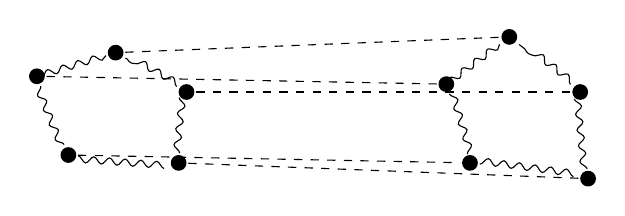
\begin{tikzpicture}[decoration = {snake,amplitude=1.2pt,segment length=2mm}]
            \fill (0,1) node (A1) {} circle (0.1);
            \fill (-1,0.7) node (A2) {} circle (0.1);
            \fill (-0.6,-0.3) node (A3) {} circle (0.1);
            \fill (0.8,-0.4) node (A4) {} circle (0.1);
            \fill (0.9,0.5) node (A5) {} circle (0.1);
            \draw[decorate] (A1)--(A2)--(A3)--(A4)--(A5)--(A1);

            \fill (5,1.2) node (B1) {} circle (0.1);
            \fill (4.2,0.6) node (B2) {} circle (0.1);
            \fill (4.5,-0.4) node (B3) {} circle (0.1);
            \fill (6,-0.6) node (B4) {} circle (0.1);
            \fill (5.9,0.5) node (B5) {} circle (0.1);
            \draw[decorate] (B1)--(B2)--(B3)--(B4)--(B5)--(B1);

            \draw[dashed] (A1)--(B1);
            \draw[dashed] (A2)--(B2);
            \draw[dashed] (A3)--(B3);
            \draw[dashed] (A4)--(B4);
            \draw[dashed] (A5)--(B5);
        \end{tikzpicture}
        \caption{Two interacting ring polymers with \(n=5\).}
    \end{figure}

    Identical particle exchange effects become important when the de Broglie thermal wavelengths \(\Lambda_i(T)=h/\sqrt{2\pi m_i k_B T}\) exceed the hard sphere diameters of the atoms. These effects can in principle be included by considering dimerisation, trimerisation, etc. of ring polymers (see Chandler and Wolynes). However, it is hardly ever necessary for those of us who work in chemistry departments to have to worry about them, because these effects are almost always negligible, e.g. in liquid para-hydrogen even at its melting temperature (\(13.8\unit{K}\)).






    \newpage
    \section{Ring Polymer Molecular Dynamics}
    Usually we are not just interested with the static thermal average \(\eval{A}\) of a quantum system. Instead we are interested time correlation functions.
    \begin{defn}
        The \textit{correlation function} of two observables \(A\) and \(B\) is
        \begin{equation}
            C_{AB}(t)\coloneqq\frac{1}{Z}\tr[\ee^{-\beta\hat{H}}\hat{A}\ee^{\ii\hat{H}t/\hbar}\hat{B}\ee^{-\ii\hat{H}t/\hbar}]\,.
        \end{equation}
    \end{defn}
    The rationalisation of this is that in the Heisenberg picture, the operator \(\hat{B}\) evolves as
    \begin{equation}
        \hat{B}(t)=\ee^{\ii\hat{H}t/\hbar}\hat{B}(0)\ee^{-\ii\hat{H}t/\hbar}\,,
    \end{equation}
    while the energy eigenstates are not changing, so
    \begin{align}
            C_{AB}(t)&=\frac{1}{Z}\tr[\ee^{-\beta\hat{H}}\hat{A}(0)\hat{B}(t)]\notag\\
            &=\frac{1}{Z}\sum_{\ket{n}}\expval{\ee^{-\beta \hat{H}}\hat{A}(0)\hat{B}(t)}{n}\notag \\
            &=\frac{1}{Z}\sum_{\ket{n}}\ee^{-\beta E_n}\expval{\hat{A}(0)\hat{B}(t)}{n}\notag \\
            &=\eval{A(0)B(t)}\,.
    \end{align}
    These correlation functions are useful because a lot of dynamical properties, like the diffusion coefficient, reaction rate constants and dipole absorption spectra can be related to those correlation functions by Green--Kubo relations. We need to figure out a way to calculate these correlation functions using ring polymers.

    Suppose now we have two coordinate-dependent operators \(\hat{A}\) and \(\hat{B}\) of interest, with classical ring-polymer counterparts \(\mathcal{A}_n\) and \(\mathcal{B}_n\) defined analogous to (\ref{ring_polymer_observable}). What does the \(n\to\infty\) limit of
    \begin{equation}
        \eval{\mathcal{A}_n \mathcal{B}_n}=\frac{1}{Z_n}\int\dd[n]{\vb{p}}\dd[n]{\vb{q}}\mathcal{A}_n \mathcal{B}_n \ee^{-\beta_n H_n}
    \end{equation}
    corresponds to? A naive guess would be
    \begin{equation}
        \eval{AB}\stackrel{?}{=}\lim_{n\to\infty}\eval{\mathcal{A}_n \mathcal{B}_n}\,,
    \end{equation}
    but this is actually wrong. To see this, we expand
    \begin{align}
        \eval{\mathcal{A}_n \mathcal{B}_n}&=\frac{1}{n^2}\sum_{i,j=1}^{n}\eval{A(q_i)B(q_j)}\,,
    \end{align}
    but to get \(\eval{AB}\) in the \(n\to\infty\) limit, we would need
    \begin{equation}
        \eval{AB}=\lim_{n\to\infty}\frac{1}{n}\sum_{i=1}^{n}\eval{A(q_i)B(q_i)}\,.
    \end{equation}
    These two are obviously unequal in general. Instead, rather surprisingly, the \(n\to \infty\) limit of \(\eval{\mathcal{A}_n \mathcal{B}_n}\) actually corresponds to something closely related to the correlation function.
    \begin{defn}
        The \textit{Kubo-transformed correlation function} of two observables \(A\) and \(B\) is
        \begin{equation}
            K_{AB}(t)\coloneqq\frac{1}{\beta Z}\int_{0}^{\beta}\dd{\lambda}\tr[\ee^{-(\beta-\lambda)\hat{H}}\hat{A}\ee^{-\lambda\hat{H}}\ee^{\ii\hat{H}t/\hbar}\hat{B}\ee^{-\ii\hat{H}t/\hbar}]\,.
        \end{equation}
    \end{defn}
    Let's have a closer look at what this means. In addition to the Boltzmann factor \(\ee^{-\lambda\hat{H}}\) and evolved \(\hat{B}\) operator \(\hat{B}(t)=\ee^{\ii\hat{H}t/\hbar}\hat{B}\ee^{-\ii\hat{H}t/\hbar}\) in the trace, we also have changed our \(\hat{A}\) operator by
    \begin{equation}
        \ee^{\lambda\hat{H}}\hat{A}\ee^{-\lambda\hat{H}}
    \end{equation}
    with an averaging over \(\lambda\) from \(0\) to \(\beta\) by the integral \(\frac{1}{\beta}\int_{0}^{\beta}\). Notice that this is similar to the time evolution we've done on \(\hat{B}\), but this time there is no factor of \(\ii\) in the exponent. We can interpret this as \textit{imaginary-time evolution},
    \begin{equation}
        \hat{A}(-\ii\hbar\lambda)=\ee^{\lambda\hat{H}}\hat{A}\ee^{-\lambda\hat{H}}\,.
    \end{equation}
    Hence in the Kubo-transformed correlation function, we are also averaging over the imaginary time of \(\hat{A}\) from \(t=0\) to \(t=-\ii\hbar\beta\). This allows us to compactly denote the Kubo-transformed correlation function as
    \begin{equation}
        K_{AB}(t)=\frac{1}{\beta}\int_{0}^{\beta}\dd{\lambda}\eval{\hat{A}(-i\hbar\lambda)\hat{B}(t)}\,.
    \end{equation}

    The ordinary correlation function and the Kubo-transformed one are more closely related in the Fourier domain. This is easily seen if we work in the basis of energy eigenstates. Inserting the resolution of identity operators in the energy basis,
    \begin{align}
        C_{AB}(t)&=\frac{1}{Z}\sum_{\ket{k}}\sum_{\ket{\ell}}\sum_{\ket{m}}\mel{k}{\ee^{-\beta\hat{H}}\hat{A}}{\ell}\mel{\ell}{\ee^{\ii\hat{H}t/\hbar}}{m}\mel{m}{\hat{B}\ee^{-\ii\hat{H}t/\hbar}}{k}\notag \\
        &=\frac{1}{Z}\sum_{\ket{k}}\sum_{\ket{\ell}}\sum_{\ket{m}}\ee^{-\beta E_k}\ee^{-\ii E_k t/\hbar}\ee^{\ii E_\ell t/\hbar}\delta_{m\ell}A_{km}B_{\ell k}\notag \\
        &=\frac{1}{Z}\sum_{\ket{k}}\sum_{\ket{m}}\ee^{-\beta E_k}\ee^{-\ii(E_k-E_m)t/\hbar}A_{km}B_{mk}\,.
    \end{align}
    Doing the same for the Kubo-transformed correlation function, we get
    \begin{align}
        K_{AB}(t)&=\frac{1}{\beta Z}\int_{0}^{\beta}\dd{\lambda}\sum_{\ket{k}}\sum_{\ket{\ell}}\sum_{\ket{m}}\mel{k}{\ee^{-\beta\hat{H}\ee^{\lambda \hat{H}}}\hat{A}}{\ell}\mel{\ell}{\ee^{-\lambda\hat{H}}\ee^{\ii\hat{H}t/\hbar}}{m}\mel{m}{\hat{B}\ee^{-\ii\hat{H}t/\hbar}}{k}\notag \\
        &=\frac{1}{Z}\sum_{\ket{k}}\sum_{\ket{m}}\ee^{-\beta E_k}\ee^{-\ii(E_k-E_m)t/\hbar}A_{km}B_{mk}\frac{1}{\beta}\int_{0}^{\beta}\dd{\lambda}\ee^{\lambda(E_k-E_m)}\notag\\
        &=\frac{1}{Z}\sum_{\ket{k}}\sum_{\ket{m}}\ee^{-\beta E_k}\ee^{-\ii(E_k-E_m)t/\hbar}A_{km}B_{mk}\frac{\ee^{\beta(E_k-E_m)}-1}{\beta(E_k-E_m)}\,.
    \end{align}
    It has got some extra bit comparing with the normal correlation function --- but it is dependent on \(E_k-E_m\), so we can't easily pull it out from the sum. Nice things happen if we move to the Fourier domain. We get
    \begin{align}
        \tilde{K}_{AB}(\omega)&=\int_{-\infty}^{\infty}\dd{t} \ee^{-\ii\omega t}K_{AB}(t)\notag \\
        &=\frac{1}{Z}\sum_{\ket{k}}\sum_{\ket{m}}\ee^{-\beta E_k}A_{km}B_{mk}\frac{\ee^{\beta(E_k-E_m)}-1}{\beta(E_k-E_m)}\int_{-\infty}^{\infty}\dd{t}\ee^{-\ii\omega t}\ee^{-\ii(E_k-E_m)t/\hbar}\,.
    \end{align}
    If you're familiar with Fourier transform, you should identify that this is exactly the delta function,
    \begin{equation}
        \int_{-\infty}^{\infty}\dd{t}\ee^{-\ii\omega t}\ee^{-\ii(E_k-E_m)t/\hbar}=2\pi\delta\left(\frac{E_m-E_k}{\hbar}-\omega\right)\,,
    \end{equation}
    and so
    \begin{equation}
        \tilde{K}_{AB}(\omega)=\frac{1}{Z}\sum_{\ket{k}}\sum_{\ket{m}}\ee^{-\beta E_k}A_{km}B_{mk}\frac{\ee^{\beta(E_k-E_m)}-1}{\beta(E_k-E_m)}2\pi\delta\left(\frac{E_m-E_k}{\hbar}-\omega\right)\,.
    \end{equation}
    The delta function naturally imposes the condition \(E_m=E_k+\hbar\omega\), so it reduces the double sum to a single sum,
    \begin{equation}
        \tilde{K}_{AB}(\omega)=\frac{1}{Z}\sum_{\ket{k}}\ee^{-\beta E_k}A_{km}B_{mk}\frac{1-\ee^{-\beta\hbar\omega}}{\beta\hbar\omega}2\pi\delta(0)\,.
    \end{equation}
    Now the extra factor from the integral over \(\lambda\) is independent of \(\ket{k}\), so we can pull it out from the sum
    \begin{equation}
        \tilde{K}_{AB}(\omega)=\frac{1-\ee^{-\beta\hbar\omega}}{\beta\hbar\omega}\frac{2\pi}{Z}\sum_{\ket{k}}\ee^{-\beta E_k}A_{km}B_{mk}\delta(0)\,.
    \end{equation}
    The Fourier transform of the normal correlation function is exactly the same except without this extra factor
    \begin{equation}
        \tilde{C}_{AB}(\omega)=\frac{2\pi}{Z}\sum_{\ket{n}}\ee^{-\beta E_k}A_{km}B_{mk}\delta(0)\,,
    \end{equation}
    and so
    \begin{equation}
        \tilde{K}_{AB}(\omega)=\frac{1-\ee^{-\beta\hbar\omega}}{\beta\hbar\omega}\tilde{C}_{AB}(\omega)\,.
    \end{equation}
    Notice also that in the classical limit, the energy spectrum becomes a continuum with \(\beta\hbar\omega\to 0\), and so
    \begin{equation}
        \tilde{K}_{AB}(\omega)\to \tilde{C}_{AB}(\omega)\,.
    \end{equation}
    




    \subsection{Relation to Ring Polymer Average}

    Having established what the Kubo-transformed correlation function is, let's see how it is related to the ring-polymer average of two observables.
    \begin{clm}
        The \(n\to\infty\) limit of \(\eval{\mathcal{A}_n \mathcal{B}_n}\) for the classical ring polymer is the \(t\to 0\) limit of the Kubo-transformed correlation function
        \begin{equation}
            \lim_{n\to\infty}\eval{\mathcal{A}_n \mathcal{B}_n}=K_{AB}(0)\,.
        \end{equation}
    \end{clm}
    \begin{proof}
        At \(t=0\),
        \begin{equation}
            K_{AB}(0)=\frac{1}{\beta Z}\int_{0}^{\beta}\dd{\lambda}\tr[\ee^{-(\beta-\lambda)\hat{H}}\hat{A}\ee^{-\lambda\hat{H}}\hat{B}]\,.
        \end{equation}
        Consider again Trotter-splitting the exponential of the Hamiltonians, but this time
        \begin{equation}
            \ee^{-(\beta-\lambda)\hat{H}}=\left(\ee^{-\beta\hat{H}}\right)^{\frac{\beta-\lambda}{\beta}}=\lim_{n\to\infty}\left(\ee^{-\beta_n\hat{H}}\right)^{n(1-\frac{\lambda}{\beta})}\,,
        \end{equation}
        and similarly
        \begin{equation}
            \ee^{-\lambda\hat{H}}=\lim_{n\to\infty}\left(\ee^{-\beta_n\hat{H}}\right)^{n\frac{\lambda}{\beta}}\,.
        \end{equation}
        Therefore,
        \begin{equation}
            K_{AB}(0)=\lim_{n\to\infty}\frac{1}{\beta Z_n}\int_{0}^{\beta}\dd{\lambda}\tr\left[\left(\ee^{-\beta_n\hat{H}}\right)^{n(1-\frac{\lambda}{\beta})}\hat{A}\left(\ee^{-\beta_n\hat{H}}\right)^{n\frac{\lambda}{\beta}}\hat{B}\right]\,.
        \end{equation}
        Let's consider the effect of the integral averaging over \(\lambda\): \(\frac{1}{\beta}\int_{0}^{\beta}\). There are \(n(1-\frac{\lambda}{\beta})\) pieces of \(\ee^{-\beta_n \hat{H}}\) in front of \(\hat{A}\) and \(n\frac{\lambda}{\beta}\) between \(\hat{A}\) and \(\hat{B}\). What the integral does is averaging over the number of \(\ee^{-\beta_n \hat{H}}\) pieces distributed between these two places, while making sure that there are \(n\) of them in total. When \(n\) is large, this can be replaced by the sum
        \begin{equation}
            \frac{1}{\beta}\int_{0}^{\beta}\dd{\lambda}f(\lambda)\longmapsto \lim_{n\to\infty}\frac{1}{n}\sum_{\lambda=1}^{n}f\left(\lambda\beta_n\right)\,.
        \end{equation}
        Therefore we can write
        \begin{equation}
            K_{AB}(0)=\lim_{n\to\infty}\frac{1}{n Z_n}\sum_{k=1}^{n}\tr\left[\left(\ee^{-\beta_n\hat{H}}\right)^{k}\hat{A}\left(\ee^{-\beta_n\hat{H}}\right)^{n-k}\hat{B}\right]\,.
        \end{equation}
        Now there are \(n+2\) operators in the trace. We again use the trick of inserting identity operators between them, while associating \(\hat{A}\) and \(\hat{B}\) to the \(\ee^{-\beta_n\hat{H}}\) in front of them, giving
        \begin{equation}
            \lim_{n\to\infty}\frac{1}{Z_n}\frac{1}{n}\sum_{k=1}^{n}\int\dd[n]{\vb{q}}\dots\mel{q_k}{\ee^{-\beta_n \hat{H}}\hat{A}}{q_{k+1}}\dots\mel{q_n}{\ee^{-\beta_n\hat{H}}\hat{B}}{q_1}\,.
        \end{equation}
        Another property of the trace we can exploit is its cyclic invariance. This means that we can move any slice of bra-kets at front to the end, and vice versa. This means that
        \begin{align}
            K_{AB}(0)=\int\dd[n]{\vb{q}}\dots\mel{q_k}{\ee^{-\beta_n \hat{H}}\hat{A}}{q_{k+1}}&\dots\mel{q_n}{\ee^{-\beta_n\hat{H}}\hat{B}}{q_1}\notag\\
            &=\int\dd[n]{\vb{q}}\dots\mel{q_i}{\ee^{-\beta_n \hat{H}}\hat{A}}{q_{i+1}}\dots\mel{q_{j}}{\ee^{-\beta_n\hat{H}}\hat{B}}{q_{j+1}}\dots\,,
        \end{align}
        as long as \(\abs{j-i}=k\). We average over all possible cyclic permutations of the trace --- there are \(n\) of them for each interval \(k\). This is effectively putting \(\hat{A}\) and \(\hat{B}\) into all possible slices of bra-kets. Therefore we can write
        \begin{align}
            K_{AB}(0)&=\lim_{n\to\infty}\frac{1}{Z_n}\frac{1}{n^2}\sum_{i,j=1}^{n}\int\dd[n]{\vb{q}}\dots\mel{q_i}{\ee^{-\beta_n \hat{H}}\hat{A}}{q_{i+1}}\dots\mel{q_j}{\ee^{-\beta_n\hat{H}}\hat{B}}{q_{j+1}}\dots\notag\\
            &=\lim_{n\to\infty}\frac{1}{Z_n}\int\dd[n]{\vb{p}}\dd[n]{\vb{q}}\mathcal{A}_n \mathcal{B}_n \ee^{-\beta_n H_n}\notag\\
            &=\lim_{n\to\infty}\eval{\mathcal{A}_n \mathcal{B}_n}\,,
        \end{align}
        which is exactly what we claimed.\qed


    \end{proof}




\end{document}